\documentclass[10pt,twocolumn,letterpaper]{article}

\usepackage{cvpr}
\usepackage{times}
\usepackage{epsfig}
\usepackage{graphicx}
\usepackage{amsmath}
\usepackage{amssymb}

% Include other packages here, before hyperref.
\newcommand{\rak}[1]{{\color{red}{rak: #1}}}
\newcommand{\ma}[1]{{\color{purple}{ma: #1}}}
\newcommand{\mgm}[1]{{\color{cyan}{mgm: #1}}}

% If you comment hyperref and then uncomment it, you should delete
% egpaper.aux before re-running latex.  (Or just hit 'q' on the first latex
% run, let it finish, and you should be clear).
\usepackage[breaklinks=true,bookmarks=false]{hyperref}

\cvprfinalcopy % *** Uncomment this line for the final submission

\def\cvprPaperID{****} % *** Enter the CVPR Paper ID here
\def\httilde{\mbox{\tt\raisebox{-.5ex}{\symbol{126}}}}

% Pages are numbered in submission mode, and unnumbered in camera-ready
%\ifcvprfinal\pagestyle{empty}\fi
\setcounter{page}{4321}
\begin{document}

%%%%%%%%% TITLE
\title{DREU Final Report: Compositional Spatio-Temporal Reasoning}

\author{Madeleine Grunde-McLaughlin\\
University of Pennsylvania\\
%Philadelphia, Pennsylvania\\
{\tt\small mgrund@sas.upenn.edu}
% For a paper whose authors are all at the same institution,
% omit the following lines up until the closing ``}''.
% Additional authors and addresses can be added with ``\and'',
% just like the second author.
% To save space, use either the email address or home page, not both

\and
Ranjay Krishna\\
Stanford University\\
%Palo Alto, California\\
{\tt\small ranjay.krishna@gmail.com}

\and
Maneesh Agrawala\\
Stanford University\\
%Palo Alto, California\\
{\tt\small maneesh@cs.stanford.edu}


}
\maketitle
\pagestyle{empty}

%%%%%%%%% ABSTRACT
\begin{abstract}
    \mgm{THIS IS AN OLD VERSION!!!!}
    Existing Video Question Answering benchmarks are limited in the spatio-temporal reasoning skills they measure. We build a pipeline to combine Action Genome's spatio-temporal scene graph annotations with predefined templates to create a new benchmark AGQA. AGQA's question templates create questions that test a wide variety of spatio-temporal reasoning skills, including action sequencing, complex temporal localization, and compositional reasoning \mgm{re-think this list and what is included}. Along with these questions, AGQA contributes an extensive suite of metrics to measure model's accuracy at different reasoning challenges, ability to generalize to new combinations of ideas, and consistency of an underlying worldview \mgm{delete consistency of underlying?}. We plan to test existing models on this new benchmark to measure their relative strengths and weaknesses. \mgm{replace with new info}
    %\rak{Needs a 1 sentence summary of why existing methods suck. Setup the problem before you say your solution.}
    %We contribute a large Video Question Answering dataset and a suite of metrics to test a wide variety of concepts. Our pipeline for automatically generating questions from spatio-temporal scene graphs creates a set of questions that explore temporal reasoning in a wide variety of ways \rak{Too vague. What are these ways?}. Our questions also focus on compositional reasoning and localizing specific sections of a video with action references. To measure performance on this task, we create a suite of metrics beyond a general accuracy score to measure a model's abilities on different types of questions, success at generalization tasks, and the consistency of its worldview.
    %\rak{The format I like to use for abstracts is: problem statement, insight/contribution statement. contribution \#2, contribution \#3, main experimental takeaways. For you, these will translate over to 1) why do existing benchmarks suck? 2) the insight that a spatio-temporal reasoning benchmark can be generated using Action Genome's scene graphs. 3) contribution \#2 is a set of question types/templates that each test for different spatio-temporal capabilities. 4) contribution \#3 is a set of new metrics that test for various abilities like compositional reasoning, temporal ordering, etc. 5) contribution \#4 is running existing video question answering models on this new benchmark. 5) main experimental takeaway is how existing video question answering models all suck at this benchmark (you might not have that for the DREU report).}
\end{abstract}

%%%%%%%%% BODY TEXT


\section{Introduction}

%\rak{paragraph 1 comments: There are some leaps in logic between the sentences in this paragraph. Sentence 1 says we need to reason. Sentence 2 talks about how actions are a hierarchy. Sentence 3 talks about spatio-temporal reasoning. These ideas are all connects but unless you draw the connections, it will leave most readers unfamiliar with what you are trying to convey.}
%The ability to perceive and reason about human activity has been a long standing goal for Computer Vision. Research in Cognitive Science suggests that humans decompose actions into a hierarchy of parts \cite{zacks2001events, ji2020action}. Therefore, in order to reason about activities, models should be capable of spatial and temporal reasoning over a subject's changing relationships with objects \cite{ji2020action}. One task developed to measure visual reasoning abilities is Visual Question Answering (VQA), in which a model answers questions about a visual input. \rak{Paragraph ends by saying VQA was introduced. I am unsure what the purpose of this paragraph is. In fact, if you start the introduction from the second paragraph, it still makes sense as a whole. This is mainly a style/preference but I like to end my first paragraphs with a problem. Make a statement about what is missing or wrong or insufficient.}
%\rak{We should create a name for the benchmark so that people can remember it and refer to it. I usually try to keep things consistent when naming. So something like Action Genome Question Answering (AGQA), pronounced aqua, benchmark?}

The ability to perceive and reason about the world's actors, actions, objects, and relationships has been a longstanding goal for Computer Vision. Formally, we can benchmark progress towards this goal using tasks like question answering, in which a model's reasoning skills are evaluated by it's ability to answer questions about visual stimuli. A variety of benchmarks have been created to test a model's capabilities at answering questions about images~\cite{johnson2017clevr,hudson2019gqa,antol2015vqa,zellers2019recognition,goyal2017making,krishna2017visual,zhu2016visual7w,kim2020answering} and about videos~\cite{tapaswi2016movieqa,lei2018tvqa,jang2017tgif,kim2017deepstory,xu2017video,maharaj2017dataset,zeng2016leveraging,yu2019activitynet}. Ideally, models trained on these benchmarks should be capable of reasoning over both spatial relationships between objects~\cite{krishna2017visual,lu2016visual} and temporal ordering of actions~\cite{zacks2001events,ji2020action}. Unfortunately, since most question-answering benchmarks operate over images, they are limited to only testing spatial relationships (e.g.~``What is on top of the table?'')~\cite{hudson2019gqa,krishna2017visual,antol2015vqa}. The few existing video-only benchmarks have questions with simple temporal logic (e.g.~``What does the bear on right do after sitting?'')~\cite{jang2017tgif,xu2017video,maharaj2017dataset,zeng2016leveraging,yu2019activitynet}. \mgm{Think I need more detail here, or when i bring it in later. Add in cleverer and commonsense reasoning} However, to answer questions that require models to jointly compose spatial and temporal reasoning over multiple steps (e.g.``What did they do to the last object they put down before opening the window?''), we need newer benchmarks and a new class of models.

%\mgm{I th ink this paragraph is much more focused than before, which is good. However, we are not going (goal -- state of world -- problem). Instead, we're saying (goal -- problem -- state of world) (with the exception of the idea that most are image-based). The current logical progression makes sense to me, but do you think there should be a more explicit "state of the world" sentence before going into the problems?}\rak{Good question. I was hoping that state of the world is image-based and the video descriptions are just problems. I think we can do a little better. I want to set the problem up so that the answer is the first sentence of the next paragraph. We want the answer to the problem to be a compositional spatio-temporal reasoning benchmark.}

We introduce the video question answering benchmark Action Genome Question Answering (AGQA) and use it to evaluate models on compositional spatio-temporal reasoning. AGQA measures a wider variety of spatio-temporal reasoning skills than existing benchmarks. An ideal benchmark to measure spatio-temporal reasoning abilities should (1) be free of human annotation bias, (2) use videos of various lengths as input, (3) contain a large number of questions, and (4) provide not just a single accuracy score but a suite of metrics that test various spatio-temporal capabilities. To achieve these goals, we developed an automatic approach that converts Action Genome’s spatio-temporal scene graphs, containing objects, relationships, actors, and actions, into compositional questions~\cite{ji2020action}. \mgm{this list came from the HAI thing, but I'm less convinced now on how important 2-3 are to bring up here. May want to bring up compositionality more explicity since we've pivoted a bit towards that, but also I'll need to have results probably that show that more compositional questions are harder.}

%First, an ideal benchmark should test questions requiring a variety of spatio-temporal \rak{stick to spatio-temporal over temporal} reasoning skills, but c

Existing question-answering benchmarks are limited in the diversity of their questions. Since most benchmarks are image-based, they only test a model's reasoning over spatial relationships~\cite{johnson2017clevr,hudson2019gqa,antol2015vqa,goyal2017making,krishna2017visual,zhu2016visual7w}, object attributes~\cite{johnson2017clevr,hudson2019gqa, antol2015vqa,goyal2017making,krishna2017visual}, and common sense understanding~\cite{zellers2019recognition,antol2015vqa,krishna2017visual}. These benchmarks are unable to test reasoning over temporal relationships or activities. \mgm{clearer common sense specification here}
%Even though a few video-based question answering benchmarks have been proposed~\cite{tapaswi2016movieqa,lei2018tvqa,jang2017tgif,kim2017deepstory,xu2017video,maharaj2017dataset,zeng2016leveraging,yu2019activitynet}, several of these prominent benchmarks rely on dialogue and plot summaries to reason over the contents of the videos~\cite{lei2018tvqa, tapaswi2016movieqa, kim2017deepstory}. Models trained on these datasets have demonstrated a stronger dependence on the dialogue input than on the visual input, reducing these benchmarks' effectiveness at measuring visual spatio-temporal reasoning~\cite{tapaswi2016movieqa,lei2018tvqa}. Therefore, our project focuses pure video-only question answering benchmark. 
The questions asked by VideoQA benchmarks that do not include extra textual information like dialogue can be answered from a single frame of the video, apply to the entire video with no temporal localization, or ask "what happened before/after/while $<$action$>$?"~\cite{jang2017tgif,xu2017video, maharaj2017dataset, zeng2016leveraging, yu2019activitynet}. \mgm{a very clunky way of bringing this up. However, I'm not sure how to do it more clearly yet. Think} Temporal localization refers to using the phrase "before/after/while $<$action$>$" to localize a relevant time in the video over which to reason. Beyond the three types of questions listed above, models should be able to perform more complex temporal localization, follow the changing state of objects over time, sequence actions, compare temporal qualities like length among different parts of the video (e.g. "Which activity did they do the longest?"), and generalize to new domains~\cite{lake2018generalization,vatashsky2020vqa}. \mgm{re-address this list with the templates we ended up with} Creating this diverse range of questions has previously been difficult. Questions automatically generated from video captions often lack diversity in structure~\cite{yu2019activitynet, jang2017tgif}. Human annotated datasets are too expensive to get a large enough sample to include a wide variety of categories~\cite{zeng2016leveraging, yu2019activitynet}
% Note to self - double check zeng talks abotu this
%Humans are able to learn quickly by generalizing new information in existing contexts \cite{tani2014self, schulz2016probing}. Improving a model's ability to generalize will allow it to more quickly learn new domains, categories, and logical rules \cite{lake2018generalization, vatashsky2020vqa}. 
The community does not know how existing models perform on more complex temporal reasoning and generalization to new content because existing benchmarks do not have questions requiring these abilities. By recursively generating questions with direct references, indirect references, and temporal localizations, our question generation pipeline creates a diverse set of questions that can be trained and tested all together or separated by type. \mgm{making the same pont like 50 different times I want to restructure it a bit to condense all that into one area b/c now it kinda rambles}

%Creating this diverse range of questions has previously been difficult. Questions automatically generated from video captions often lack diversity in structure \cite{yu2019activitynet, jang2017tgif}. Human annotated datasets are too expensive to get a large enough sample to include a wide variety of categories, and benchmark creators have limited control over the contents of each question, limiting the ability to break down the test set into relevant categories \mgm{is what we say about human annotators true? I wanted to address the difficulties for each type, but I have not found anything relevant for human annotators}\rak{I think you just want to say something simpler - that it would take a lot of money to generate a dataset with the same size since each video-question pair will cost money.}. By recursively generating questions with direct references, indirect references, and temporal localizations, our question generation pipeline creates a diverse set of questions that can be trained and tested all together or separated by type. \rak{You have setup three wonderful points in the paragraph where I said goosebumps but your first point took up 3 paragraphs. You need to simply these into 1 paragraph and only get the main message across. You can divide deeper in the related work section. Intro should be high level and related work and make more specific distinctions.}

%\mgm{seems like the above section is too long and makes this ideal benchmark list lose continuity. How can I condense the first point?}
An ideal VideoQA benchmark measures the ability to reason over visual stimuli instead of depending on the statistics of answer distributions~\cite{vatashsky2020vqa}. However, many question answering datasets have a bias towards common answers that reduce dependence on visual input and inflate accuracy scores~\cite{goyal2017making, hudson2019gqa}. 
%It is difficult for existing benchmarks to smooth answer distributions because they do not have direct access to structural and semantic content to separate them into granular categories. \mgm{I wanted to include the "Why is this hard" point. However, no vision-only video datasets tried even on the categories they did have. Should I just leave it as "this has not yet been done" or extrapolate why it may be difficult?} 
Since we have question content information from our generation pipeline, we are able to smooth the answer distribution among different question types. \mgm{ideally add in numbers about how that makes the blind model worse but idk}
%\rak{You want to draw on how for tasks like object detection and image classification, people often try to balance their dataset and then talk about why it's difficult to do for your task.} TODO: FOR THE FINAL PAPER DO THIS!!!

An ideal VideoQA benchmark would have videos with a variety of video lengths. Some VideoQA datasets have a variety of clip lengths~\cite{yu2019activitynet,xu2017video}, but most VideoQA datasets use videos of less than 10 seconds long~\cite{jang2017tgif,kim2017deepstory,xu2017video,maharaj2017dataset,zeng2016leveraging,yu2019activitynet}. Some models are better suited for longer or shorter videos, but an ideal model would be able to reason over a variety of lengths~\cite{na2017read,le2020hierarchical}. Although it is expensive to annotate longer clips, we use two already annotated datasets on videos from 2.33 to 194.33 seconds long~\cite{sigurdsson2016hollywood,ji2020action}. \mgm{questionable how important this is, though it is true}

An ideal VideoQA benchmark should be large. All current VideoQA sets have less than 350K question answer pairs~\cite{jang2017tgif,kim2017deepstory,xu2017video,maharaj2017dataset,zeng2016leveraging,yu2019activitynet,lei2018tvqa,tapaswi2016movieqa}. A larger training set can support a wider variety of questions while avoiding underfitting, and a larger testing set can be split into a wider variety of subsets~\cite{maharaj2017dataset}. On only 250 videos, our process generated over 8 million questions of diverse structures. Our final dataset will generate questions on over 9.8K videos. \mgm{no longer as impressively large - probably take out}

Finally, an ideal VideoQA benchmark provides a wide range of metrics to judge a model's relative strengths and weaknesses. Most existing benchmarks measure accuracy on the overall dataset~\cite{maharaj2017dataset,jang2017tgif,xu2017video,maharaj2017dataset,zeng2016leveraging,yu2019activitynet}. Some also measure accuracy on categories of questions~\cite{jang2017tgif,xu2017video,yu2019activitynet}, or on questions without visual input~\cite{zeng2016leveraging}. For example~\cite{xu2017video} splits questions by the first word ("what", "where", "who", "how, "when"). %, and \cite{jang2017tgif} splits the test set into 1) questions that look at the number of times an action was performed, 2) questions naming the action that occurred X times, 3) questions that use temporal localization, and 4) questions that could be answered from one frame. \mgm{Are these examples helpful or just confusing?}
Reasoning complexly about videos requires multi-step reasoning, comparative and counting operators, flexibility with video length, appearance feature understanding, and fine and coarse motion understanding~\cite{le2020hierarchical,fan2019heterogeneous}. The accuracy scores of existing benchmarks do not provide the granularity needed to measure success in these different aspects of video understanding~\cite{fan2019heterogeneous,le2020hierarchical}. Furthermore, no existing benchmarks we know of measures a model's ability to generalize to new information. AGQA provides a suite of new metrics measuring accuracy by category, the ability to generalize, and the extent to which a model's answers reflect a consistent and realistic understanding of the world. \mgm{Will need to adjsut this based on the metrics that I got done. For example, didn't do entailments which was the crux of the "consistent worldview" part. So I probbaly want to shift the focus to measuring compositional reasoning}

We have made much progress within the DREU timeline working towards creating a benchmark that has these qualities, and we plan to continue the project through the fall. This final report discusses the questions for 250 videos, generating over 8 million question and answer pairs. By the end of our project, our contributions will be: 1) a large VideoQA dataset of question answer pairs requiring multi-step reasoning and 2) a wide suite of metrics to thoroughly evaluate current models. \mgm{delete this part and replace with model results}


%\subsection{Old introduction}


%First, to control dataset bias we smooth the distribution of answers such that models cannot simply rely on linguistic bias and must consider the visual input. 
%Second, to test for the human-like capacity to understand visual concepts as novel combinations of a set of core objects and relationships~\cite{ji2020action, tani2014self} we recursively generate questions by combining basic logical operations that operate over objects and relationships in the video (see Figure~\ref{fig:example}).
%Third, to test different types of spatio-temporal reasoning we divide the benchmark into multiple splits. Some splits test models' capability to generalize to novel question compositions, some measure the ability to transfer from questions that require fewer logical steps to those that require longer compositional operations, and some test for few-shot reasoning over concepts that appear only a few times during training.
%After generating this benchmark, we will test existing video question answering models on the numerous subsets and report which capabilities are displayed by existing methods and which underperform.



%\rak{For what reason? Because they are different than images? I would argue the oppositve. People didn't work on videos because they are more than images. Instead, I would argue that people worked on images because it was simpler than videos and we have always wanted to only work on videos.} For this reason, a growing number of VideoQA benchmarks have been released, but current benchmarks exhibit some weaknesses \rak{cite papers in the sentence where you make claims}.

%First, many involve short videos ($<$ 10 seconds) \cite{jang2017tgif, kim2017deepstory, xu2017video, maharaj2017dataset}, or contain fewer than 200k questions \cite{tapaswi2016movieqa, lei2018tvqa, kim2017deepstory, xu2017video, jang2017tgif, yu2019activitynet, zeng2016leveraging}. \rak{It is true that existing datasets use short videos and are smaller. But you need to tell the reader why that matters? Why are larger benchmarks better?}

%Second, current benchmarks require at most two reasoning steps to answer. For example, the question "What happened to the woman before playing violin?" requires first finding when the woman played violin, then looking at what happened before then \cite{yu2019activitynet}). \rak{Again, you need to setup what you actually want to accomplish before explaining how existing methods aren't good enough. Without having a north star, it's hard to understand why we care about having logical and comparative questions in benchmarks.} However, few questions require more steps of reasoning and refined temporal localization than that example.  Existing benchmarks also do not use logical or comparative operators in their questions, which leaves out interesting and relevant ideas (e.g. "Which activity did they do for longer?"). Since many VideoQA models get stuck when faced with questions that require multiple reasoning steps, leaving out these questions limits current benchmarks  \cite{fan2019heterogeneous}. \rak{I don't think we need newer benchmarks because models can't do something. Models' also can't raise an ant farm but we aren't trying to develop benchmarks for developing ant farms. Instead, you want to argue the opposite --- we want models that can do X because people expect them to. But to train models that can do X and evaluate them, we need a benchmark. Current benchmarks suck because they don't measure these tenents of X.}

%Third, several of these benchmarks integrate visual cues with dialogue and plot summaries \cite{lei2018tvqa, tapaswi2016movieqa, kim2017deepstory}. Their analysis found that question answering models depend more heavily on the dialogue input than on the visual input, reducing these benchmarks' effectiveness at measuring visual temporal reasoning \cite{tapaswi2016movieqa, lei2018tvqa}. 

%Fourth, after the release of the first large ImageQA datasets, investigations found that their answer distributions were heavily skewed. This bias towards very common answers effectively reduces dependence on visual input and inflates accuracy scores \cite{goyal2017making, hudson2019gqa}. Some ImageQA datasets have worked to balance answer distributions \cite{goyal2017making, hudson2019gqa}, but to our knowledge no VideoQA datasets have systematically balanced answer distributions. \rak{You are going back to talking about image QA datasets in the middle of talking about videoQA ones. It breaks the flow of your argument.}

%Finally, existing benchmarks have accuracy measurements only for the overall dataset and for each question type (e.g. Repetition Count, Repeating Action, State Transition, and Frame-based questions in \cite{jang2017tgif}). Reasoning about videos requires multi-step reasoning, comparative and counting operators, flexibility with video length, appearance feature understanding, and fine and coarse motion understanding. A wider metrics suite would improve measurement of models' relative strengths and weaknesses across these many categories.

%We propose a VideoQA benchmark that addresses these concerns. Our benchmark is automatically generated in a pipeline inspired by \cite{hudson2019gqa} to combine question templates with Charades action annotations and Action Genome's spatio-temporal scene graphs. This process combines a variety of linguistic structures with the content of over 10,000 videos. These questions have a wide variety of lengths, complexities, and structures. With this generation pipeline, we have tight control over the contents of each question, allowing us to balance the answer distribution and create a wide suite of metrics.

%We have made much progress within the DREU timeline, and we plan to continue the project through the fall. This final report discusses the questions for 250 videos, generating over 8 million question and answer pairs. By the end of our project, our contributions will be: 1) a large VideoQA dataset of question answer pairs requiring multi-step reasoning and 2) a wide suite of metrics to thoroughly evaluate current models.

%\rak{Overall - I think you have all the points in there. You have everything that needs to be said or explaind. They just need to be reshuffled to follow a logical argument. Currently, to draw a terrible analogy, you are moving your queen into position before setting up the knight to defend the queen. You bring up imageQA multiple times in the introduction but it's not clear why it matters. Similarly, you bring up all the problems with videoQA but don't setup what is the ideal benchmark.

%My second high level suggestion would be to pick a reasonable audience. Right now, it feels like you are writing for VQA and videoQA researchers. But other computer vision researchers or ML researchers in general might not understand why your criticism of existing work matters. Remember that most people have not read all the papers you have you have. I find it useful to write for a version of myself before I began working on a project. So, try writing for Madeleine in May, who hadn't read all these papers in detail.

%I would suggest going back to the HAI grant we wrote and thinking about the structure we introduced there. You should be able to use that exact grant and make it the first 3 paragraphs of your introduction.}

\section{Prior Work}



\subsection{ImageQA}

At first, the Visual Question Answering task was mostly restricted to ImageQA. A wide variety of benchmark datasets were created with the hopes of analyzing the reasoning abilities of ImageQA models~\cite{johnson2017clevr,hudson2019gqa,antol2015vqa,zellers2019recognition,goyal2017making,krishna2017visual,zhu2016visual7w,kim2020answering}. Benchmarks vary in input, from synthetic datasets~\cite{johnson2017clevr}, to cartoons~\cite{antol2015vqa}, to charts~\cite{kim2017deepstory}, to real-world images~\cite{hudson2019gqa,krishna2017visual,zhu2016visual7w,goyal2017making,zellers2019recognition,antol2015vqa}. They also vary in the type of questions asked, from descriptive 7W's (who, what, where, when, which, why, how)~\cite{zhu2016visual7w}, to commonsense reasoning~\cite{zellers2019recognition}, to compositional reasoning~\cite{johnson2017clevr,hudson2019gqa}, to spatial localization~\cite{zhu2016visual7w,krishna2017visual,hudson2019gqa}. These benchmarks facilitated the development of many models made to tackle these challenges by measuring their spatial reasoning abilities~\cite{johnson2017clevr,hudson2019gqa,krishna2017visual,vatashsky2020vqa}. \mgm{replace these citations}%TOFO: should probs just find plain models \mgm{re}

However, many of these datasets contained real world priors exacerbated by human annotation bias, resulting in inflated accuracy scores and a lack of understanding of the actual reasoning abilities of these models~\cite{goyal2017making,hudson2019gqa}. For example, in the VQA1.0 dataset, 41\% of answers  for questions starting with "What sport is..." were "Tennis". These types of priors meant that models could answer over 50\% of the questions correctly without considering the visual input~\cite{goyal2017making}. Once these issues came to light, some new benchmarks attempted to mitigate these biases. VQA2.0 took many of the questions from VQA1.0 and added a similar picture leading to a different answer. This procedure helped, but was only applied to 71\% of questions due to annotation difficulties. Models measured on VQA2.0 could still answer 67\% of binary questions and 27\% of open answer questions correctly without seeing visual input~\cite{hudson2019gqa} \mgm{our open answer blind model is similar.. so this point is less salient unless we can bring that down}. The GQA dataset addressed these biases by smoothing the answer distribution by question category. This balancing of the answer distribution retains but reduces the power of real world priors ~\cite{hudson2019gqa}. AGQA is similar to GQA in that it mitigates biases by smoothing answer distributions. However, it will move beyond just spatial reasoning and into the temporal domain. 

\subsection{VideoQA}

A growing interest in Visual Question Answering has also lead to the development of some VideoQA benchmarks~\cite{tapaswi2016movieqa,lei2018tvqa,jang2017tgif,kim2017deepstory,xu2017video,maharaj2017dataset,zeng2016leveraging,yu2019activitynet}. Several of these prominent benchmarks rely on dialogue and plot summaries to reason over the contents of videos~\cite{lei2018tvqa,tapaswi2016movieqa,kim2017deepstory}. Models trained on these datasets have demonstrated a stronger dependence on the dialogue input than on the visual input, reducing these benchmarks' effectiveness at measuring visual spatio-temporal reasoning~\cite{tapaswi2016movieqa,lei2018tvqa}. Therefore, our project focuses pure video-only question answering benchmark. 

%\mgm{order this paragraph more like the intro}
Vision-only benchmarks exclusively ask questions that can be answered from a single frame of the video, questions that apply to the entire video with no temporal localization, or questions that ask "what happened before/after/while $<$action$>$?". They all, except~\cite{yu2019activitynet,xu2017video}, refer to videos of less than 10 seconds long.  Some have automatically generated questions from image descriptions~\cite{xu2017video,zeng2016leveraging}, some let human annotators choose from drop down menus~\cite{jang2017tgif}, and others ask humans annotators to create questions~\cite{yu2019activitynet,tapaswi2016movieqa,jang2017tgif,lei2018tvqa}. The largest dataset with solely human generated questions is~\cite{lei2018tvqa} with 152.5K question answer pairs, and the largest dataset with solely automatically generated questions is~\cite{maharaj2017dataset} with 349K question answer pairs. Our dataset is purely vision based, works on videos of 2-195 seconds long, and evaluates complex and multi-step temporal reasoning. \mgm{Very mch a laundry list of kist x y z. Maybe will do They are x, we are y. They are a, we are b structure? Otherwise take out less indteresting stuff}

\begin{figure}[t]
\begin{center}
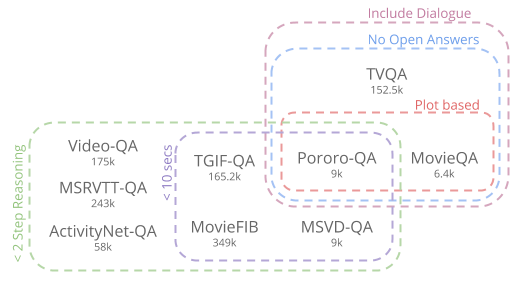
\includegraphics[width=0.8\linewidth]{Figures/figure_videoQA.png}
\end{center}
   \caption{Existing VideoQA benchmarks have some drawbacks. Specifically, many have questions with less than 2 steps of reasoning, using short videos, having plot based questions, only multiple choice questions, and including dialogue.}
\label{existing_benchmarks}
\end{figure}

%Expanding question-answering to videos has been gaining interest lately \mgm{passive voice and bad sentence}, and a small number of datasets have been produced. Some of these datasets incorporate both visual input and dialogue from a TV show or Movie \cite{}, and several of which ask plot-based, not exclusively vision based questions \cite{}. This is an important task, but since models based on these datasets tend to depend heavily on dialogue for long-term temporal reasoning \cite{}, our benchmark will focus on purely visual temporal reasoning. Of current benchmarks doing purely visual temporal reasoning, all but \cite{} refer to videos of less than 10 seconds long. Futhermore, all of them reason in simple (change wording) ways over time \cite{}. These are limited to x, y, z, frame based. MSRVTT-QA is also mostly 2 types of questions. Our dataset will be purely vision based, work on videos of 30-90 seconds long, and require a model to perform complex temporal reasoning. 


\subsection{Compositional Reasoning}

As questions become more complex, they often require multiple reasoning steps in order to find the answer. For example, the question "Was the person running or sitting for longer?" first requires finding the start and end of when the person was running and sitting, subtracting the start from the end, then comparing the lengths of each action's occurrence. A constrained set of logical steps (e.g. action localization, subtraction, comparison, etc) can be used as building blocks that are reordered to respond to a wide variety of different questions. This multi-step reasoning is called compositional reasoning because the overall understanding is composed of a series of smaller reasoning steps. Humans are able to learn quickly by generalizing new information in existing contexts~\cite{tani2014self,schulz2016probing}. Improving a model's ability to generalize will allow it to more quickly learn new domains, categories, and logical rules~\cite{lake2018generalization,vatashsky2020vqa}. 


\begin{figure}[t]
\begin{center}
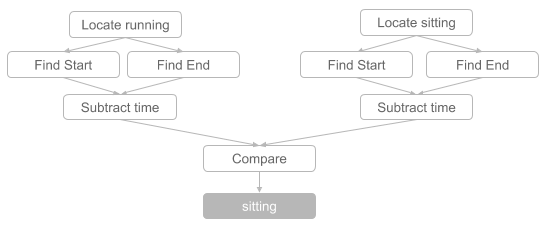
\includegraphics[width=0.8\linewidth]{Figures/figure_composition.png}
\end{center}
   \caption{The substeps required to answer the question "Was the person running or sitting for longer?"}
\label{compositional_substeps}
\end{figure}



Compositional questions have been used by ImageQA benchmarks to rigorously test models. Compositional questions tend to be longer, more complex, and use a wider variety of vocabulary. Furthermore, they can better test a model's reasoning ability both by requiring multiple steps of reasoning to answer the questions and by allowing for datasets to test generalization to novel compositions~\cite{johnson2017clevr,hudson2019gqa,lake2018generalization}. For example, on the CLEVR dataset, the training questions could include the phrases "right of cube" and "behind sphere", but not "right of sphere" as a combination. Testing on this novel combination "right of sphere" in the test set tests a model's ability to generalize to new concepts~\cite{lake2018generalization,johnson2017clevr}. Many questions relevant to reasoning over videos require multi-step reasoning. A simple example covered by current datasets involves first localizing in time, then reasoning about that specific time. For example, this question from~\cite{jang2017tgif}, "What does the model do after
lower coat?", requires finding when the model lowers her coat, then determining her activity after that. Another way to reason compositionally is to refer to subjects indirectly, as the ImageQA benchmark~\cite{hudson2019gqa} does with "What color is the food on the red object to the left of the girl?". 

Some ImageQA benchmarks use compositional reasoning extensively~\cite{johnson2017clevr,hudson2019gqa}, but no VideoQA datasets go beyond two steps of compositional reasoning. Although these logical building block steps have been defined for ImageQA~\cite{cheng2015break}, there are no compositional reasoning steps defined for temporal reasoning. Current models have struggled with multi-step reasoning, motivating a benchmark like ours that specifically explores compositional reasoning~\cite{fan2019heterogeneous}. \mgm{Think this has the right information, though may switch back and forth between different types of things (multistep vs novel combination) so I want to be clearer in how I structure it}


\subsection{Scene Graphs}

Scene graphs are a symbolic representation of an image~\cite{krishna2017visual}. The graph consists of nodes representing the objects in the image and edges representing relationships between those objects. For each object node there are associated attributes. For example, an image with a man wearing white shorts would have an object node for "shorts" with "white" as an attribute and an object node for "man". These object nodes would be connected by an edge representing the relationship "wearing". Creating this symbolic representation of an image reduces it to its semantic parts. Using this representation has improved performance on many visual tasks such as visual question answering~\cite{johnson2017inferring}, visual question answer generation~\cite{hudson2019gqa}, relationship modeling~\cite{krishna2018referring}, image captioning~\cite{anderson2016spice}, image generation~\cite{johnson2018image,ashual2019specifying}, and image retrieval ~\cite{ashual2019specifying,johnson2015image}.

Inspired by Visual Genome's scene graphs,~\cite{ji2020action} annotated spatio-temporal scene graphs to create Action Genome. Spatio-temporal scene graphs consist of nodes representing objects and edges representing relationships between them. Each of these objects are associated with a specific frame in the video. The resulting effect is that a subject's relationships with the objects changes over time. Our project will use these spatial-temporal scene graphs to generate questions about videos. \mgm{Does the strcuturing of related work sections matter? this seems like an anti-climatic one to end on}

\mgm{Related work generally: I'm not sure how relevant all the parts are. CLEVR talks about how it balances answers and b/c its synthetic can do more in depth reasoning abilities. GQA talks about balancing answers and how CLEVR is synthetic, and other synthetic question generation methods. So i think focusing more of this section on the previous balancing attempts would help. I'm not sure how important the distinction between ImageQA and VideoQA is. Also neither of them split up the Related work into subsections.}

\section{Related Work New Attempt}

\subsection{Visual Question Answering}
1st paragraph: talk about VQA and briefstatement how ours is different

\subsection{Synthetic Datasets}
2nd paragraph: synthetic datasets. How previous synthetic for VideoQA not great, but our method more similar to VQA and CLEVER. Esp b/c its natural for videos etc

\subsection{Balancing Question-Answering Datasets}
3rd paragraph: like vqa and clevr, we also balance the dataset. Can talk abotu the benefits of this and how (double check) other videoqa don't besides cleverer. and we make sure individuals are 50/50

\subsection{Compositional Reasonign}
4th compositiona reasoning: a part of videos, but less explicitly explored or ddemanded



\section{Methods}

\subsection{Types of Temporal Reasoning}
To create AGQA, we first established what types of temporal reasoning to explore. As mentioned previously, other vision-based VideoQA datasets have looked exclusively at questions that could be answered with one frame, questions that refer to the entire video with no temporal localization, and questions that ask "what happened" before, after, or while an event was occurring~\cite{tapaswi2016movieqa,lei2018tvqa,jang2017tgif,kim2017deepstory,xu2017video,maharaj2017dataset,zeng2016leveraging,yu2019activitynet}. \mgm{again, clunky way of describing}

%\begin{itemize}
%	\item action sequencing
%	\item When actions precede, suceed, or coexist with one another
%	\item lengths of time activities occured
%	\item Reasoning about a subject's changing relationship with objects
%	\item Reasoning beyond action recognition after localizing within the video \mgm{does this make sense to normal people?}
%	\item comparative and logical operators 
%\end{itemize}

However, there are more types of temporal reasoning yet to be explored and tested on models. These new types include action sequencing, reasoning over the length of time activities occurred, reasoning with comparative and logical operators, reasoning more deeply over a subject's changing relationship with objects over time, and reasoning about when actions precede, succeed, or coexist with one another.  \mgm{re-address this list}

%Finally, after localizing in time (e.g. before running), existing benchmarks do not require reasoning beyond action recognition, so other questions could require different types of 

% reasoning over a specified part of a video instead of just action recognition. \mgm{rewrite sentence} Since activities are composed of a subject's changing relationship with objects, questions can ask about those changes. Questions should also probe action sequencing and understanding ordering of actions within the video and when actions precede, succeed or coexist with one another. Current datasets do not ask questions about the lengths of time activities occurred. Beyond temporal reasoning, current VideoQA datasets do not do comparitive or logical (i.e. "and", "xor") questions. 
 
AGQA requires all the above types of reasoning to succeed. \mgm{can I back that up?} Future datasets may be able to expand even further by including questions with sequences, bounding boxes, and time identifiers (e.g. she started running at 10.5 seconds) as answers. \mgm{keep this in conclusion?}

\begin{figure}[t]
\begin{center}
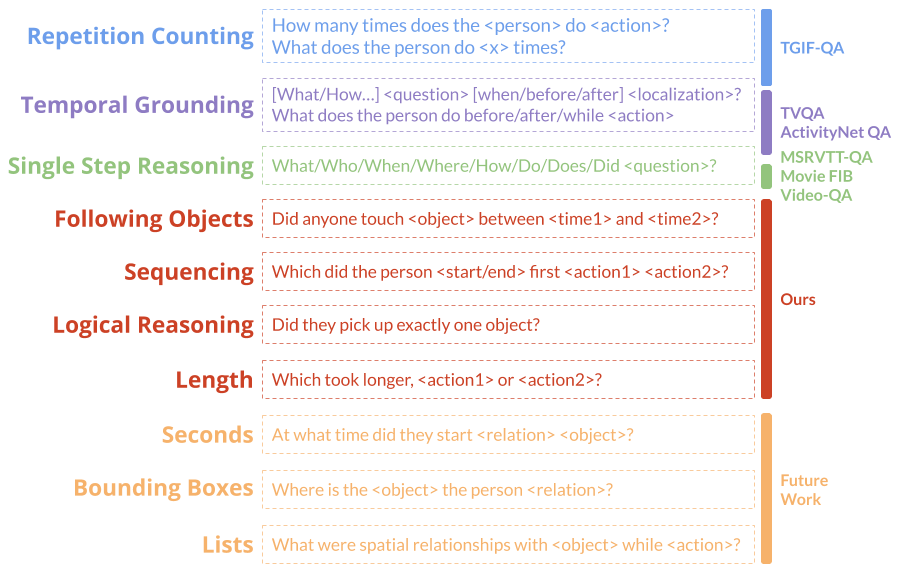
\includegraphics[width=0.8\linewidth]{Figures/figure_temporalTypes.png}
\end{center}
   \caption{Various types of temporal reasoning.}
\label{temporal_types}
\end{figure}


\subsection{Our Generation Pipeline}
Beyond exploring a wider variety of temporal concepts, an ideal benchmark would be large, mitigate biases in the answer distribution, allow for novel compositions and include a large suite of metrics. In order to achieve these goals, we automatically generate questions using a pipeline inspired by~\cite{hudson2019gqa}.
% TODO: in the future, make this match the introduction

The question generation pipeline consists of two parts: 1) augmenting spatio-temporal scene graphs to create detailed video representations and 2) building question templates with spaces for video-specific content. The first part of our pipeline uses dataset annotations from Action Genome and Charades~\cite{ji2020action,sigurdsson2016hollywood} on Charades videos. These videos are 30 seconds long on average and filmed by non-professionals \mgm{MTurk workers} who act out everyday activities using 36 objects. Charades annotates the times actions occur, and Action Genome annotates objects and attention, spatial, and contact relationships on a sample of frames. 

To make these scene graphs applicable for question answering, we first combine the annotations from both datasets into one data structure. We created object and relationship nodes for action segmentation, adding in Charades actions as a relationship category. We then supplement current annotations with their logical extensions. For example, if a person is carrying something, they are also holding it and touching it. With these adjustments, we have a filled out detailed spatio-temporal scene graphs combining two datasets worth of annotations into a structure that can be fed into the question templates. An important limitation to note is that although these scene graphs are detailed, our questions depend on their annotations, so any errors in those datasets affects our own. \mgm{add in more detail about action priors and combining multiply annotated objects and other things like this}
    
The second part of our pipeline consists of question templates that each have a natural language sentence with tags representing different elements categories in the video, such as in the question "What were they $<$contact relationship$>$?". These tags can be objects, relationships, actions, or temporal localization phrases (e.g. "before putting down the dish"). Each template also contains information about the question's structural and semantic contents. 

To generate a question-answer pair, our system combines a spatio-temporal scene graph with these templates by replacing the tags with elements of the corresponding types. For a video where the person is holding a blanket while sitting on a chair, our pipeline would create both questions "What were they holding?" and "What were they sitting on?". Given the scene graph information, we then automatically determine the answers "blanket" and "chair" respectively. 

These tags can be filled with both direct and indirect references. For example, an $<$object$>$ tag's direct reference would be "blanket" but an indirect reference would be "the object they were holding". We ensure that there are no questions that give away the answers (e.g. "Were they holding the object they were holding?"). Indirect references can also be recursive. The object tag noted above could also be replaced with "the object they were holding after closing the door" or "the object they were holding after the shortest action". Indirect references require locating the referred object, action, relationship, or time in video before reasoning about the question as a whole, leading to complex questions that require multiple reasoning steps. 
    
    
\begin{figure*}[t]
\begin{center}
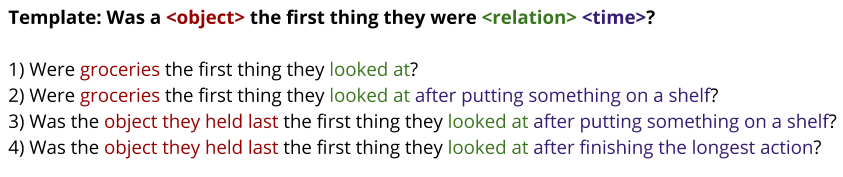
\includegraphics[width=0.8\linewidth]{Figures/figure_indirect.png}
\end{center}
   \caption{Our pipeline uses indirect references to create a variety of questions with different required reasoning steps from the same template. 1) uses all direct references and no temporalization. It has two steps of reasoning (determining if looked at groceries, then finding if that is the first thing at which they looked). 2) Adds temporal localization for a total of 4 steps (localizing when putting something on a shelf, then shifting attention after). 3) Uses an indirect reference for the object, adding one additional step (the last object held) for a total of 5 steps. 4) adds an indirect reference within the temporal localization to add a step (find the longest action) for a question with a total of 6 compositional steps required to answer.}
\label{template_expansion}
\end{figure*}

\begin{figure*}[t]
\begin{center}
%\fbox{\rule{0pt}{2in} \rule{.9\linewidth}{0pt}}
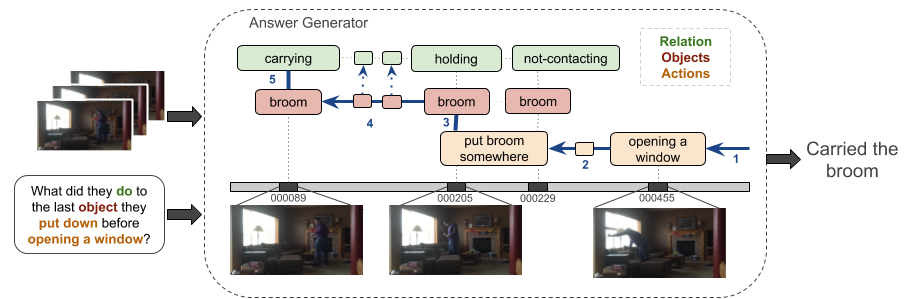
\includegraphics[width=0.8\linewidth]{Figures/figure_questionGenerator.png}
\end{center}
   \caption{The sequence in which our answer generator traverses the spatio-temporal scene graph to automatically generate the answer to a question. The input question can be decomposed into the following spatio-temporal operations: 
  1) localize when the actor opened a window, 
  2) find the last event before then when the actor put an object down, 
  3) determine which object (the broom) was put down, 
  4) look for a different relationship between the actor and this broom, 
  5) Output that the actor ``carried the broom''.}
\label{answer_generator}
\end{figure*}



This procedure to generate questions allows us to work towards the qualities of an ideal benchmark. \mgm{If I change this in the beginning may need to chang this here}
    
\subsection{Large}
    
    Human annotation of question-answer pairs for video is time consuming and expensive. Automatically generating questions allows us to create a much larger dataset of 8 million questions on just 250 videos. Automatically generated datasets have previously been criticized for lacking diversity~\cite{yu2019activitynet}. We have 32 templates asking a wide variety of questions. Each template is also associated with multiple natural language versions of the same question. Indirect reference tags expand complexity even further. \mgm{need to upate the number of templates. It's really unimpressive atm though}

\subsection{Mitigates Biases in Answer Distribution}
    
    Many ImageQA benchmarks do not accurately determine a model's reasoning ability because skews in their answer distributions reduce dependence on visual input and increase reliance on the relative prevalence of different answers in the data~\cite{hudson2019gqa,goyal2017making}. Although there has not been an in depth analysis of skewed answer distributions in Video QA biases, our dataset, if left unbalanced, would be skewed. For example, a person is covered by a blanket 6721 times but standing on a blanket only 32 times. Consequently, the answer to the question "What were they doing to the blanket?" is much more likely to be "covered by" rather than "standing on". To avoid inflated accuracy scores, we want to retain the same distribution (i.e. still have more instances where the answer is "covered by"), but smooth the answer distribution to make the differences less extreme. We balance the answer distribution for each category using the same process as~\cite{hudson2019gqa} to downsample highly popular answers to shift probability into the tail of the distribution. Our question generation pipeline allows for this balancing because we have the structural and semantic information associated with each template to split the questions into relevant categories before downsampling. 

    \mgm{need to explain this in more detail and update it with the new way that I've been doing it. }
    
   \subsection{Novel Composition Tests}
    
    An important part of human reasoning is the ability to generalize concepts of the same category to novel compositions. For example, in the training set the model may see the phrases "before running" and "the action they did the longest". Then, in the test set, we can test if they understand the idea of "before the action they did the longest". We are able to create such a training and testing split to judge these novel compositions because we have knowledge of what temporal localization, logical reasoning, and indirect tags are in each question.
    
    \mgm{Add in more detial about other compositional tests as well. Also, maybe some more detail into how I make the compositinal tests}

    \subsection{Suite of New Metrics}
    
    Finally, we want to be able to complexly analyze a model's various abilities across different types of temporal and logical reasoning. We can achieve better measurements by choosing different subsets of questions from the training and test sets. We are able to do this because our pipeline gives us control over the content of all the questions. 
    
    \mgm{Will create a whole section about this. I'll probably put it in the analysis section instead}
    
    At the end of the 10 weeks of the DREU program, we have not yet balanced the dataset's open answer questions or divided the questions into a suite of metrics. However, we plan to incorporate these steps by the end of the summer. 

\section{Results}

A the end of the 10 weeks of DREU, we have generated 8 million questions from 32 templates and 250 videos. Our final Video QA dataset consists of three parts: the Charades videos, without any annotations or the corresponding spatio-temporal scene graphs, the questions, the answers, and the suite of metrics. 

In other words, AGQA = $\{ V, Q, A, M \}$, where every $v_i \in V$ corresponds to a list of questions $q_i  \in Q$ and a list of corresponding answers $a_i \in A$. For every question $q_{ij} \in q_i$ there is a corresponding answer $a_{ij} \in q_i$. $M$ is a suite of metrics specifying which questions from the training and test set should be included to get a score for each metric. \mgm{neither clevr or gqa really rescribe it like this}


Figure \ref{answer_dist} shows that, like other question-answering datasets, our answer distribution has a very long tail. We plan to mitigate the effects of this long tail by balancing the distribution of answers for each category. 

Certain question templates generate many more questions than others. Across the 250 videos, the template that asks "Did they $<$relation$>$ a $<$object1$>$ or a $<$object2$>$?" generates over 2,138,702 questions, while the template that asks "What is the last thing they did to the $<$object$>$ only generates 345 questions. This disparity occurs because there are many more permutations to fill in all 4 tags of the first question than the 1 tag in the second question. Furthermore, many videos do not have a valid object to fill into the second question, because the person is doing multiple things to the object at once. The questions with the most answers are yes/no questions, so this disparity is also reduced through balancing. 

Figure \ref{steps} shows that we have a large number of compositional steps in many of our questions. Our method of counting is described in more detail in Figure \ref{template_expansion}. The highest number of compositional steps in a single template is 5, suggesting that many questions gain additional compositionality from indirect references. These results show we have generated complex questions with many compositional steps. 


\mgm{Add this information, in a condensed form, to the end of the dataset generation section I think}

\subsection{Structural and Semantic Categories}

Following the categorizations of~\cite{hudson2019gqa} we break down the questions into structural and semantic categories. 

Structural categories define the structure of the question. We have three structures, verify, choose, and compare. \mgm{add in new ones} Verify questions have "Yes" and "No" answers verifying if a question is correct (e.g. Did they carry the blanket?). Choose questions choose between two answers (e.g. Did they carry the blanket or the dish?). Query questions have open answers (e.g. What did they carry?). As seen in Figure \ref{structural}, there are significantly more "verify" questions than the other categories. However, this distribution will shift after balancing. For example, after balancing only 22\% of the verify questions remain. We plan to balance the other categories in the future.

Semantic categories define what ideas the question is mainly reasoning about. In our dataset, these semantic categories are objects, relationships, object-relationship pairs, and actions. As seen in Figure \ref{semantics}, the dataset consists mostly of questions asking about object-relationship pairs and objects. 

\mgm{bring structural/semantic category stuff to when describing global attributes for experiments and results}


\mgm{Overall Methods/Results notes: Clevr talks about be Image and scene representations, image generation, question representations, and question generation. GQA talks more about the question generation pipeline and is closer to what I followed here. Split into four sections 1- scene graph normalization, 2-  question representation 3- functional representation and entailment (we don't have entailment and aren't releasing the programs yet) and 4- sampling and balancing. I think instead of structuring it like i do here where it follows the qualities of the ideal benchmark (which is what we did for HAI) following a more GQA style description of each step in the question generation pipeline may make sense. However, that was also part of their contribution whereas for us, its the tool we used from their contribution. So maybe makes more sense to talk about compositional reasoning and the semantic categories (nvm include this in methods) that are time-specific. Also, I'll want to go into the balancing more specifically since I deviated some from the algorithm GQA did.  }

\setion{ Methods round 2}

Introduction talking about GQA, but how expanded out to temporal domain. 

\subsection{Spatio-temporal Scene graphs}

Expanding them out to include action genome and charades
dealing with uncertainty in action segmentation and adding in priors. Which occur at same time, which occur one before the other
Adding in commonsense entailments. I.e. if carrying also holding and touching
Fixing issues with spatial relationships such that the human becomes the subject
Augmenting AG annotations with breakdown of STSGs
Dealing with synonymous words and doubly-annotated objects by noting which are the same with IOUs and overlapping action annotations
Correlating vauge and specific things ('eating something' and 'eating some food' at same time)

\subsection{Question Templates}
Natural language variety
Different 
Only ask questions i fmultiple answers
Avoiding non-sensical questions 
Avoiding questions that give it away in the answer
Avoid common sense combos like "are they wearing clothes" that may not be annotated
Make sure no ambiguity in whcih its refering to

Each associated witha. program to automatically descern the answer
B/c pass thorugh a lot of information about the question as they are generated, able to balance and create interesting metrics. 

\subsection{Creating Compositional Reasoning}
Some in the question itself
Add in indirect references and temporal localizations
Can say balanced to make sure x\% of questions with temporal localizations changed the answer
In creating the questions, each indirect reference was associated with a program that coudl be recursively added to reason about that first

\subsection{Balancing}
Based of GQA, but went further. 

For binary, split into specific categories (xor - rel - obj - obj)
For open, first truncated less common answers. Then did the head moving forward thing until either the first x\% of answers made up less than y\% of all questions, or more than half the questions were deleted. These numbers were chosen by experiment to find the smoothest distribution that keeps some priors but works a lot better.

Did this on global, then local. Then also did it with structural type of question. THere are 5 types of question, a, b, c, d, e. Made it so the local smoothness was retained, but teh different templates used were made more smooth, and got the proportions of quesiton types ot be 50\% this, 10\% that ext. 

If balance by temporal, also do that. If keep balancing by making indirect obj ref as the same distribution, say that.


\subsection{Results}
Before balancing, was x, y, z. After balancing, was x, y, z. Figures of how the distributions changed. 


\section{Experiments and analysis - TO ADD}

CLEVR: First described models. They then analyzed the dataset by question type (query vs compare), relationship type (spatial vs attribute), question topology (chain vs tree-structured questions). they have an interesting section on looking at "effective" question size. They say that accuracy is not necessarily related to question size itself, so they prune functions from the program until they find the smallest functional program that when put on the scene graph creates the correct answer. This is the 'effective' program length, and that is related to difficulty. Nothing comes immediately to mind about how I would do that with AGQA though. They also looked at relative vs absolute spatial reasoning. SO if you say "left of x" they see how accurate it is if you just look in left half of the image, and then they prune when spatial relationships aren't absolutely necessary. They found that much worse on ones that require relative, not absolute, spatial reasoning. This could potentially be expanded to temporal localization. Then look at novel combinations. They have a summary in discussions and future work. 

GQA: breaks down semantic and structural categories (does not spend much time on these),then talks about data set's vocabulary size and possible answers. We are a lot weaker on this point. GQA talks about briefly baseline experiments on blind models. They they describe transfer performance, i.e. training on VQA and testing on GQA and vice versa to show theirs is harder (we don't have an equivalent though). Then, they get into describing their new metrics and have. subsection for each category. For some of them they have a formal representation, for others they don't.

% Note to self: will need to change some to logical structural.. maybe compare?

Notes to self: I think that the stuff CLEVR did with pruning down programs to find the essential necessities is cool. I probably don't have time for that now, but worth keeping in mind. 

Questions
1- Do we want to spend time describing the models? Should we spend any time describing the overall trends of VideoQA models? CLEVR does but GQA doesnt.
2- Do we have time to do all these metrics?
3- CLEVR said that question length did not correspond with complexity until they pruned. I don't think I have time for that now. However, is it important to bring up that it doesn't get more complex? Or could talk about how a lot more difficult when temporal localization changes the answer... Not sure how much need to motivate the compositional stuff. 
4- Should blind mode be blind of the existing models, or like blind LSTM and blind CNN? Also, do we need to do blind where just sees visual too?
5- Need to consider how much detail to go into describing structural and semantic categories. 
6- What metrics should be prioritized? Unfortunately have implemented the ones where it is necessary to use a different triaining set. Also, for novel composition, do I need to go into detail about each novel composition or can it be talked about generally? Or just have 1 example?

7- How much related work should be on the type of questions in previous datasets, vs on compositionality, vs on balancing answers. Should I add in something about synthetic datasets? Can I take out the scene graphs section?

8- How much in detail to explain the question generation process? Since GQA basically already did it. I want to focus more on the compositional part and balancing. Also, besides saying I added in qualifications and augmented the scene graphs, how much should go into describing those edits? GQA talks briefly about normalizing scene graph vocabulary. They put more detail in supplementary which might be a good plan.

Sections

\subsection{Describe the models we looked at breifly}

\subsection{Semantic and Structural and Global}

Briefly describe these categories and how we look at metrics.

Discuss experiments on blind models and results on actual models 

\subsection{Compositional metrics}

For each subsection descriibe 

\subsubsection{Novel Composition}

\subsubsection{Indirect Reference}

\subsubsection{Number of Compositional Steps}

\subsubsection{Length of video}



\subsection{}

\begin{figure}[t]
\begin{center}
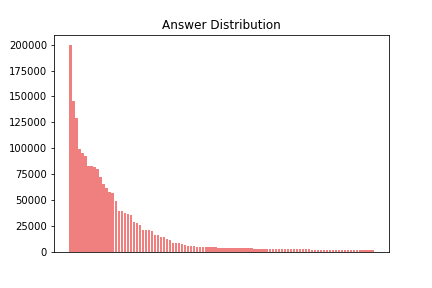
\includegraphics[width=0.8\linewidth]{Figures/answer_dist.png}
\end{center}
   \caption{The distribution of the top 100 answers (excluding "Yes" and "No").}
\label{answer_dist}
\end{figure}


\begin{figure}[t]
\begin{center}
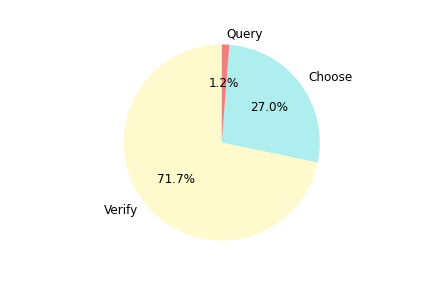
\includegraphics[width=0.8\linewidth]{Figures/struct_dist.png}
\caption{The structural distribution of questions.}
\end{center}
\label{structural}
\end{figure}


\begin{figure}[t]
\begin{center}
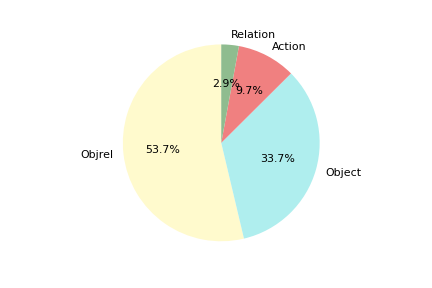
\includegraphics[width=0.8\linewidth]{Figures/sem_dist.png}
\end{center}
   \caption{The semantic distribution of questions.}
\label{semantics}
\end{figure}


\begin{figure}[t]
\begin{center}
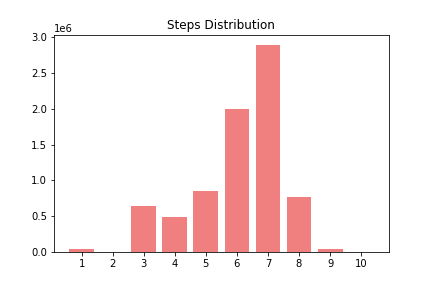
\includegraphics[width=0.8\linewidth]{Figures/steps_dist.png}
\end{center}
   \caption{The distribution of the number of compositional steps.}
\label{steps}
\end{figure}



%\begin{figure}[t]
%\begin{center}
%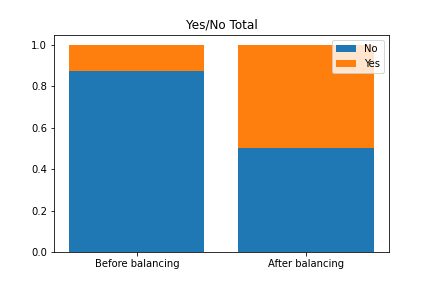
\includegraphics[width=0.8\linewidth]{Figures/yn_total.png}
%\end{center}
%   \caption{The proportion of questions with a Yes/No answer before and after balancing}
%\label{binary_balance}
%\end{figure}


\begin{table}[]
    \begin{center}
    \caption{Suite of Metrics}
    \label{metrics}
    \begin{tabular}{|p{2cm}|p{5cm}|}
     \hline
     \multicolumn{2}{|c|}{\textbf{Content Category}}\\
    \hline
    All & Accuracy on all questions\\
    \hline
    Question Type & Accuracy on each question category (e.g. Counting, Length, First, ...)\\
    \hline
    Answer Type & Accuracy on each answer category (e.g. binary, and open)\\
    \hline
    
    
     \multicolumn{2}{|c|}{\textbf{Generalization}}\\
    \hline
    Video Length & Train on videos of length $<$ 30 seconds. Test on videos of length $\geq$ 30 seconds \\
    \hline
    Actions & Train on videos with $<$ 5 actions. Test on videos with $\geq$ 5 actions  \\
    \hline
    Compositional Steps &  Train on questions with $<$ 6 steps. Test on questions with $\geq$ 6 steps  \\
    \hline
    Novel Compositions & See Table \ref{novel_composition_table} \\
    \hline
    Indirect Consistency & Accuracy on questions referring to the same ideas but using different numbers of indirect references\\
    \hline
    Direct Only & Questions with no indirect refs\\
    \hline
    \% Training Data & Train on only 1, 5, 10 and 20 percent of training data \\
    \hline
    
    
     \multicolumn{2}{|c|}{\textbf{Answer Legitimacy}}\\
    \hline
    Sequencing & Something where sequencing is consistent \\
    \hline
    Consistent & If answers a question correctly, answers all logical entailments correctly \\
    \hline
    Validity & Answer type is of correct genre (e.g. object, relation, action, count, yes/no)\\
    \hline
    Plausibility  & Answer exists in distribution for that question\\
    \hline
    Distribution & Predicted answers follow same distribution as ground truth\\
    \hline
    \end{tabular}
    \end{center}
\end{table}


\begin{table}[]
    \begin{center}
    \caption{Novel Composition}
    \label{novel_composition_table}
    \begin{tabular}{|p{2cm}|p{5cm}|}
    \hline
    \textbf{Name} & \textbf{Novel Combinations} \\
    \hline
    object-relationship & touching table, touching food, beneath table, beneath food\\
    \hline
    repetition & taking a dish from somewhere, putting some food somewhere\\
    \hline
    first/last & looking at first, behind first, holding first \\
    \hline
    before/after & before standing up, before playing with phone, before throwing broom\\
    \hline
    longer & longer than standing up, longer than playing with phone, longer than throwing broom\\
    \hline
    
    \end{tabular}
    
    \end{center}
\end{table}

\section{Future work}

To complete this project, we plan to expand upon our current progress in four ways through the fall. First, we will create a wider variety of templates, both in the subject of what they ask and in the natural language question. Second, we will balance the dataset on non-binary questions. Third, we will implement a suite of metrics. Fourth, we will evaluate existing VideoQA models on our dataset~\cite{le2020hierarchical,fan2019heterogeneous,li2019beyond}

We have already balanced the dataset for yes/no questions. We plan to smooth the distribution of all open ended questions.

We want AGQA to be able to provide a complex analysis of the abilities of VideoQA models. Therefore, we will create a suite of metrics, each of which measures a different aspect of performance, as specified in Table \ref{metrics}. Content Category metrics ask how well the model performs overall and on different question and answer categories. Generalization metrics ask if given a small portion of basic concepts, can the model generalize to more complex questions. Answer legitimacy metrics ask if the model has a consistent and plausible understanding of the contents of the video. Our suite of metrics will provide insight on these questions and a more detailed understanding of the model's strengths and weaknesses.


\section{Conclusion}
Our project automatically generates a dataset of question-answer pairs for video and a suite of metrics on which to measure performance.
AGQA will facilitate the creation of VideoQA models by providing a challenging task.

{\small
\bibliographystyle{ieee_fullname}
\bibliography{dreu_final}
}

\end{document}
